\DeclareOption*{\PassOptionsToClass{\CurrentOption}{abntex2}}
\ProcessOptions


\documentclass[
	% -- opções da classe memoir --
	12pt,				% tamanho da fonte
	openright,			% capítulos começam em pág ímpar (insere página vazia caso preciso)
	oneside,			% para impressão em verso e anverso. Oposto a oneside
	a4paper,			% tamanho do papel. 
	% -- opções da classe abntex2 --
	%chapter=TITLE,		% títulos de capítulos convertidos em letras maiúsculas
	%section=TITLE,		% títulos de seções convertidos em letras maiúsculas
	%subsection=TITLE,	% títulos de subseções convertidos em letras maiúsculas
	%subsubsection=TITLE,% títulos de subsubseções convertidos em letras maiúsculas
	% -- opções do pacote babel --
	english,			% idioma adicional para hifenização
	french,				% idioma adicional para hifenização
	spanish,			% idioma adicional para hifenização
	brazil				% o último idioma é o principal do documento
	]{abntex2}

%sudo apt update
%sudo apt install texlive-latex-extra (instalar pacote abntex2)

\usepackage{abntex2}
	
%%%%%%%%%%%%%%%%%%%%%%%%%%%%%%%%%%%%%%%%%%%%%%%%%%%
% conf-comandos.sty
%%%%%%%%%%%%%%%%%%%%%%%%%%%%%%%%%%%%%%%%%%%%%%%%%%%
	
\ProvidesPackage{conf-comandos}

% ----------------------------------------------------------
% Imprimir a ficha catalográfica
% ----------------------------------------------------------
\newcommand{\imprimirficha}[1]{
    \begin{fichacatalografica}
        \includepdf{#1}
    \end{fichacatalografica}
}

% ----------------------------------------------------------
% Imprimir a folha de aprovação
% ----------------------------------------------------------
 %\providecommand{\imprimirtextoaprovacao}{}
% \newcommand{\textoaprovacao}[1]{
%     \renewcommand{\imprimirtextoaprovacao}{
%         \begin{center}#1\end{center}
%     }
% } 
% \newcommand{\imprimiraprovacao}{
%     \begin{folhadeaprovacao}
%         \begin{center}
%             \ABNTEXchapterfont\SingleSpacing\bfseries\Large\MakeUppercase\imprimirtitulo
%             \vspace*{2.0cm}
            
%             \ABNTEXchapterfont\normalsize\bfseries\MakeUppercase\imprimirautor
%             \vspace*{1.0cm}
%         \end{center}
        
%         \noindent\OnehalfSpacing\imprimirtextoaprovacao
        
%         \vspace*{1.0cm}
%         \begin{center}    
%             \imprimirlocal, 19 de abril, 2021.
%         \end{center}
        
%         \noindent Banca Examinadora:
        
%         \assinatura{\imprimirorientador, Dr. Eng.} 
% %        \assinatura{\imprimircoorientador, Dr.}
%         \assinatura{Matheus Leitzke Pinto, Msc.}
%         \assinatura{Gustavo Martins de Araújo Silvano, Eng.
            
%         }
%     \end{folhadeaprovacao}
% }

% ----------------------------------------------------------
% Imprimir a folha de dedicatória
% ----------------------------------------------------------
\newcommand{\imprimirdedicatoria}[1]{
    \begin{dedicatoria}
        \vspace*{\fill}
        \begin{flushright}
        \noindent
        \textit{#1}
        \vspace*{2cm}
        \end{flushright}
    \end{dedicatoria}
}

% ----------------------------------------------------------
% Imprimir a lista de códigos
% ----------------------------------------------------------
\newcommand{\listoflistings}{
    \begin{KeepFromToc}
        \lstlistoflistings
    \end{KeepFromToc}
}

% ----------------------------------------------------------
% Imprimir a lista de abreviaturas
% ----------------------------------------------------------
\newcommand{\sortitem}[2]{%
    \DTLnewrow{sortlist}%
    \DTLnewdbentry{sortlist}{sig}{#1}% 
    \DTLnewdbentry{sortlist}{desc}{#2}% 
}

\newenvironment{sortsiglas}{%
    \DTLifdbexists{sortlist}{\DTLcleardb{sortlist}}{\DTLnewdb{sortlist}}%
}{%
    \DTLsort{sig}{sortlist}% Sort list
    \begin{siglas}%
        \DTLforeach*{sortlist}{\theDesc=desc, \theSig=sig}{\item[\theSig] \theDesc}% Print each item
    \end{siglas}%
}%

\makeatletter

% \abreviatura{abrev.}{definição}
% ret = 
\newcommand{\abreviatura}[2]{%
    \write\@auxout{\noexpand\@writefile{abrv}{\noexpand\sortitem{#1}{\xmakefirstuc{#2}}}}%
}%

% \abreviatura*{abrev.}{definição}
% ret = abrev. (definição)
\WithSuffix\newcommand\abreviatura*[2]{%
    #1 (#2)%
    \write\@auxout{\noexpand\@writefile{abrv}{\noexpand\sortitem{#1}{\xmakefirstuc{#2}}}}%
}%

% \abreviatura.{abrev.}{definição}
% ret = definição (abrev.)
\WithSuffix\newcommand\abreviatura.[2]{%
    #2 (#1)%
    \write\@auxout{\noexpand\@writefile{abrv}{\noexpand\sortitem{#1}{\xmakefirstuc{#2}}}}%
}%

% \abreviatura'{abrev.}{definição}{tradução}
% ret = 
\WithSuffix\newcommand\abreviatura'[3]{%
    \write\@auxout{\noexpand\@writefile{abrv}{\noexpand\sortitem{#1}{\textit{#2} - \xmakefirstuc{#3}}}}%
}%

% \abreviatura&{abrev.}{definição}{tradução}
% ret = tradução (definição - abrev.)
\WithSuffix\newcommand\abreviatura&[3]{%
    #3 (\textit{#2} - #1)%
    \write\@auxout{\noexpand\@writefile{abrv}{\noexpand\sortitem{#1}{\textit{#2} - \xmakefirstuc{#3}}}}%
}%

\newcommand{\imprimirlistadeabreviaturas}{%
    \begin{sortsiglas}%
        \@starttoc{abrv}%
    \end{sortsiglas}%
}%
\makeatother

% ----------------------------------------------------------
% Imprimir a lista de simbolos
% ----------------------------------------------------------
\newenvironment{sortsimbolos}{%
    \DTLifdbexists{sortlist}{\DTLcleardb{sortlist}}{\DTLnewdb{sortlist}}%
}{%
    \DTLsort{desc}{sortlist}% Sort list
    \begin{simbolos}%
        \DTLforeach*{sortlist}{\theDesc=desc, \theSig=sig}{\item[\theSig] \theDesc}% Print each item
    \end{simbolos}%
}%

\makeatletter

% \simbolo{simbolo}{definição}
% ret = 
\newcommand{\simbolo}[2]{%
    \write\@auxout{\noexpand\@writefile{asbl}{\noexpand\sortitem{#1}{\xmakefirstuc{#2}}}}%
}%

% \simbolo*{simbolo}{definição}
% ret = simbolo
\WithSuffix\newcommand\simbolo*[2]{%
    #1%
    \write\@auxout{\noexpand\@writefile{asbl}{\noexpand\sortitem{#1}{\xmakefirstuc{#2}}}}%
}%

\newcommand{\imprimirlistadesimbolos}{%
    \begin{sortsimbolos}%
        \@starttoc{asbl}%
    \end{sortsimbolos}%
}%
\makeatother

% ----------------------------------------------------------
% Imprimir a fonte da figura
% ----------------------------------------------------------
\newcommand{\indentedfont}[2][\textwidth]{%
    \captionsetup{singlelinecheck=off,width=#1}%
    \caption*{\raggedright\footnotesize\mdseries Fonte: #2.}%
}%

% ----------------------------------------------------------
% Incluindo códigos que estão em um arquivo externo
% ----------------------------------------------------------
\newcommand{\includecode}[4][c]{
    \lstinputlisting[captionpos=t,caption=#3, label=#2,escapechar={@*}, style=#1]{#4}
}
%-- \includecode[linguagem]{label}{Titulo}{arquivo}
%-- \includecode[shell]{l_olamundo}{Olá mundo em shell script}{codigos/ola.sh}




% ----------------------------------------------------------
% Comandos para organizar a escrita
% ----------------------------------------------------------
% alterar | alterado | nota | add
\newcommand{\marcador}[2]{%
%
    \def\param{#1}%
    \def\ifalterar{alterar}%
    \def\ifalterado{alterado}%
    \def\ifnota{nota}%
    \def\ifadic{add}%
%
	\ifx\param\ifalterar%
		\textcolor{red}{#2}%
	\else%
		\ifx\param\ifalterado%
	        \textcolor{blue}{#2}%
	    \else%
        	\ifx\param\ifnota%
		        \textcolor{OliveGreen}{#2}%
            \else%
                \ifx\param\ifadic%
    		        \textcolor{Fuchsia}{#2}%
                \else%
                    \textcolor{black}{#2}%
                \fi%
            \fi%
        \fi%
	\fi%
}%

\WithSuffix\newcommand\marcador*[3]{%
%
    \def\param{#1}%
    \def\ifalterar{alterar}%
    \def\ifalterado{alterado}%
    \def\ifnota{nota}%
    \def\ifadic{add}%
%
	\ifx\param\ifalterar%
		\textcolor{red}{\underline{#2}} \textcolor{Mahogany}{(#3)}%
	\else%
		\ifx\param\ifalterado%
		    \textcolor{blue}{\underline{#2}} \textcolor{NavyBlue}{(#3)}%
	    \else%
        	\ifx\param\ifnota%
        	    \textcolor{OliveGreen}{\underline{#2}} \textcolor{Green}{(#3)}%
            \else%
                \ifx\param\ifadic%
            	    \textcolor{Fuchsia}{#2} \textcolor{Mulberry}{(\underline{#3})}%
                \else%
                    \textcolor{black}{\underline{#2}} \textcolor{gray}{(#3)}%
                \fi%
            \fi%
        \fi%
	\fi%
}%

\begin{comment}
    % Abreviatura em pt
    \abreviatura{abrev.}{definição}  -> ret: 
    \abreviatura*{abrev.}{definição} -> ret: abrev. (definição)
    \abreviatura.{abrev.}{definição} -> ret: definição (abrev.)
    % Abreviatura em língua estrangeira
    \abreviatura'{abrev.}{definição}{tradução} -> ret:
    \abreviatura&{abrev.}{definição}{tradução} -> ret: tradução (abrev. - definição)
    
    \simbolo{simbolo}{definição}  -> ret: 
    \simbolo*{simbolo}{definição} -> ret: simbolo
    
    \marcador{tipo}{texto}             -> ret: texto
    \marcador*{tipo}{texto}{alteração} -> ret: texto (alteração)
        alterar     | alterado  | nota      | add
        Vermelho    | Azul      | Verde     | Roxo
    
    \indentedfont{tamanho}{texto} -> ret: Fonte: texto.
    
    \includecode[linguagem]{label}{Titulo}{arquivo}
\end{comment}


%%%%%%%%%%%%%%%%%%%%%%%%%%%%%%%%%%%%%%%%%%%%%%%%%%%
% conf-ifsc.sty
%%%%%%%%%%%%%%%%%%%%%%%%%%%%%%%%%%%%%%%%%%%%%%%%%%%

% !TEX root = monografia.tex

\ProvidesPackage{conf-ifsc}

\usepackage{conf-pacotes}
\usepackage{conf-comandos}
\usepackage{tocloft}

% ----------------------------------------------------------
% Macros
% ----------------------------------------------------------
\newcommand{\buck}{Buck \textit{interleaved}}

% ----------------------------------------------------------
% Configuração do pacote de SI
% ----------------------------------------------------------
\sisetup{detect-all} % Configura fonte do pacote siunitx
\sisetup{output-decimal-marker = {,}}
\sisetup{mode = text, detect-italic = true}

% ----------------------------------------------------------
% Configuração das figuras
% ----------------------------------------------------------
\newlength{\imagewidth}  % the name can be chosen, e.g. picwidth...
\captionsetup[figure]{font={footnotesize,bf}}
\captionsetup[table]{font={footnotesize,bf}}

% ----------------------------------------------------------
% Definicao da geometria da página - Conforme Norma para TCC IFSC
% ----------------------------------------------------------
\RequirePackage[
    inner=3.0cm,
    outer=2.0cm,
    top=3.0cm,
    bottom=2.0cm,
    head=0.7cm,
    foot=0.7cm
    ]{geometry}

% ----------------------------------------------------------
% ..........................................................
% CONFIGURAÇÕES DE PACOTES
% ..........................................................
% ----------------------------------------------------------

% ----------------------------------------------------------
% Fontes padroes de part, chapter, section, subsection e subsubsection
% ----------------------------------------------------------
\renewcommand{\familydefault}{\sfdefault}             % Fonte Arial

\renewcommand{\ABNTEXchapterfont}{\sffamily}
\renewcommand{\ABNTEXchapterfontsize}{\normalsize\scshape\bfseries}

\renewcommand{\ABNTEXpartfont}{\ABNTEXchapterfont}
\renewcommand{\ABNTEXpartfontsize}{\ABNTEXchapterfontsize}

\renewcommand{\ABNTEXsectionfont}{\ABNTEXchapterfont}
\renewcommand{\ABNTEXsectionfontsize}{\normalsize\bfseries}

\renewcommand{\ABNTEXsubsectionfont}{\ABNTEXsectionfont}
\renewcommand{\ABNTEXsubsectionfontsize}{\normalsize}

\renewcommand{\ABNTEXsubsubsectionfont}{\ABNTEXsubsectionfont}
\renewcommand{\ABNTEXsubsubsectionfontsize}{\normalsize\itshape}

%\renewcommand{\ABNTEXsubsubsubsectionfont}{\ABNTEXsubsectionfont}
%\renewcommand{\ABNTEXsubsubsubsectionfontsize}{\normalsize}



\renewcommand{\cftpartleader}{\cftdotfill{\cftdotsep}} 
\renewcommand{\tocpartapendices}{                
    \addtocontents{toc}{\vspace{-0.6cm}}         
    \addtocontents{toc}{\cftsetindents{part}{\cftlastnumwidth}{2em}}          
    \cftinserthook{toc}{A}     
}

\renewcommand{\tocpartanexos}{
    \addtocontents{toc}{\vspace{-0.6cm}}
    \addtocontents{toc}{\cftsetindents{part}{\cftlastnumwidth}{2em}}
    \cftinserthook{toc}{A}
}
 
 
 
 
% ----------------------------------------------------------
% Fontes das entradas do sumario
% ----------------------------------------------------------
\renewcommand{\cftpartfont}{\bfseries\normalsize}
\renewcommand{\cftpartpagefont}{\bfseries\normalsize}

\renewcommand{\cftchapterfont}{\bfseries}
\renewcommand{\cftchapterpagefont}{\normalsize\cftchapterfont}

\renewcommand{\cftsectionfont}{\bfseries}
\renewcommand{\cftsectionpagefont}{\cftsectionfont}

\renewcommand{\cftsubsectionfont}{\normalsize}
\renewcommand{\cftsubsectionpagefont}{\cftsubsectionfont}

\renewcommand{\cftsubsubsectionfont}{\textit}
\renewcommand{\cftsubsubsectionpagefont}{\cftsubsubsectionfont}

\renewcommand{\cftparagraphfont}{\footnotesize}
\renewcommand{\cftparagraphpagefont}{\cftparagraphfont}


% ----------------------------------------------------------
% Remover cabeçalho nas paginas pares
% ----------------------------------------------------------
\makepagestyle{parpage}
\makeevenhead{parpage}{\ABNTEXfontereduzida\thepage}{}{}
\makeoddhead{parpage}{\ABNTEXfontereduzida\rightmark}{\rule[-.3\baselineskip]{\linewidth}{.4pt}}{\ABNTEXfontereduzida\thepage}

% ----------------------------------------------------------
% Configuração de espaçamento 
% ----------------------------------------------------------
\setlength{\afterchapskip}{0.5cm}   % Espaço 1,5 após os capítulos
\setlength{\parindent}{2.0cm}       % Identação do paragrafo conforme norma para TCC IFSC
\setlength{\parskip}{0.1cm}         % Controle do espaçamento entre um parágrafo

% ----------------------------------------------------------
% Configurações do pacote backref
% ----------------------------------------------------------
%\renewcommand{\backrefpagesname}{Citado na(s) página(s):~}
%\renewcommand{\backref}{}       % Texto padrão antes do número das páginas
%\renewcommand*{\backrefalt}[4]{ % Define os textos da citação
%	\ifcase #1 
%		Nenhuma citação no texto.
%	\or
%		Citado na página #2.
%	\else
%		Citado #1 vezes nas páginas #2.
%	\fi
%}

\def\UrlLeft{}
\def\UrlRight{}

% --------------------------------------------------------------------------
% Personalização do modelo da abnTeX2 para se adequar com o modelo do IFSC
% 2017-08-23 - Segue o modelo do IFSC publicado em setembro de 2016
% --------------------------------------------------------------------------

% ----------------------------------------------------------
% Alteração da capa
% ----------------------------------------------------------
\renewcommand{\imprimircapa}{
    \begin{capa}
        \begin{SingleSpacing}
            \center
            \ABNTEXchapterfont\bfseries\ INSTITUTO FEDERAL DE EDUCAÇÃO, CIÊNCIA E TECNOLOGIA DE\\SANTA CATARINA - CÂMPUS FLORIANÓPOLIS\\DEPARTAMENTO ACADÊMICO DE SAÚDE E SERVIÇO\\CURSO DE MESTRADO PROFISSIONAL EM CLIMA E AMBIENTE
            
            \vspace*{3.0cm}
            
            \ABNTEXchapterfont\bfseries\imprimirautor
        
            \begin{vplace}[0.5]
                \begin{center}
                    \ABNTEXchapterfont\SingleSpacing\bfseries\imprimirtitulo
                \end{center}
            \end{vplace}
            \begin{figure}[h]
    	\centering
    	
\includegraphics[scale=0.12]{figuras/ifsc.jpg}
    \end{figure}
    \\
    \vspace*{2.5cm}
            \begin{center}
                \ABNTEXchapterfont\bfseries\imprimirlocal, \ABNTEXchapterfont\bfseries\imprimirdata
            \end{center}
        \end{SingleSpacing}
    \end{capa}
}

% ----------------------------------------------------------
% folha de rosto 
% ----------------------------------------------------------
\makeatletter
\renewcommand{\folhaderostocontent}{
    \begin{SingleSpacing}
        \center
        \ABNTEXchapterfont\bfseries\ INSTITUTO FEDERAL DE EDUCAÇÃO, CIÊNCIA E TECNOLOGIA DE\\SANTA CATARINA - CÂMPUS FLORIANÓPOLIS\\DEPARTAMENTO ACADÊMICO DE SAÚDE E SERVIÇO\\CURSO DE MESTRADO PROFISSIONAL EM CLIMA E AMBIENTE
        
        \vspace*{3.0cm}     % três espaços simples - conforme norma para TCC do IFSC
        
        \ABNTEXchapterfont\bfseries\imprimirautor
        
        %\begin{vplace}[0.5]
        \vspace*{\fill} 
            \begin{center}
                \ABNTEXchapterfont\SingleSpacing\bfseries\imprimirtitulo
            \end{center}
        \vspace*{\fill} 
        %\end{vplace}
        
        \hspace{.45\textwidth}
        \begin{minipage}{.5\textwidth}
            \begin{SingleSpacing}
                \normalfont\imprimirpreambulo
                \vspace*{1.0cm}

                \imprimirorientadorRotulo~Prof. \imprimirorientador\par
                 \vspace*{1.0cm}
                \imprimircoorientadorRotulo~ \imprimircoorientador%
                
            \end{SingleSpacing}
        \end{minipage}%
        \vspace*{\fill}

         \begin{center}
            \ABNTEXchapterfont\bfseries\imprimirlocal, \ABNTEXchapterfont\bfseries\imprimirdata
        \end{center}
    \end{SingleSpacing}
}
\makeatother


% ----------------------------------------------------------
% Configurações de aparência do PDF final
% ----------------------------------------------------------
\definecolor{blue}{RGB}{41,5,195}   % alterando o aspecto da cor azul

\makeatletter
\hypersetup{                        % informações do PDF
     %	pagebackref=true,
		pdftitle={\@title}, 
		pdfauthor={\@author},
    	pdfsubject={\imprimirpreambulo},
		pdfkeywords={Palavra chave 1}{Palavra chave 2}{Palavra chave 3}, 
		colorlinks=true,       		% false: boxed links; true: colored links
    	linkcolor=black,          	% color of internal links
    	citecolor=black,        		% color of links to bibliography
    	filecolor=black,      		% color of file links
		urlcolor=black,
		bookmarksdepth=4
}
\makeatother

% ----------------------------------------------------------
% compila o indice
% ----------------------------------------------------------
\makeindex 

% --------------------------------------------------------------------------
% Configurações para inserir código fonte de programas - pacote listings
% --------------------------------------------------------------------------

\renewcommand{\lstlistingname}{Código} % Altera o nome padrão do rótulo usado no comando \autoref{}
\renewcommand{\lstlistlistingname}{Lista de códigos} % Altera o rótulo a ser usando no elemento pré-textual

% ----------------------------------------------------------
% Configura a "Lista de Códigos" conforme as regras da ABNT
% ----------------------------------------------------------
\begingroup\makeatletter
\let\newcounter\@gobble\let\setcounter\@gobbletwo
  \globaldefs\@ne \let\c@loldepth\@ne
  \newlistof{listings}{lol}{\lstlistlistingname}
  \newlistentry{lstlisting}{lol}{0}
\endgroup

\renewcommand{\cftlstlistingaftersnum}{\hfill--\hfill}

\let\oldlstlistoflistings\lstlistoflistings
\renewcommand{\lstlistoflistings}{
   \begingroup
   \let\oldnumberline\numberline
   \renewcommand{\numberline}{\lstlistingname\space\oldnumberline}
   \oldlstlistoflistings
   \endgroup
}

% ----------------------------------------------------------
% Definindo cores
% ----------------------------------------------------------
\definecolor{hellgelb}{rgb}{1,1,0.9}
\definecolor{colKeys}{rgb}{0,0,0}
\definecolor{colIdentifier}{rgb}{0,0,0.9}
\definecolor{colComments}{rgb}{.4,.4,.4}
\definecolor{colString}{rgb}{0,0,0.6}

\definecolor{colBack}{rgb}{1,1,.98}
\definecolor{colKeys}{rgb}{0,0,0}
\definecolor{colIdentifier}{rgb}{0,0,0.9}
\definecolor{colComments}{rgb}{.4,.4,.4}
\definecolor{colString}{rgb}{0,0,0.6}

\lstset{ %
    aboveskip=\bigskipamount,
    backgroundcolor=\color{colBack},   % choose the background color; you must add \usepackage{color} or 
    basicstyle=\ttfamily\footnotesize,       % the size of the fonts that are used for the code
    breakatwhitespace=false,         % sets if automatic breaks should only happen at whitespace
    breaklines=true,                 % sets automatic line breaking
    captionpos=n,                    % sets the caption-position to bottom
    columns=flexible,
    commentstyle=\color{colComments},    % comment style
    deletekeywords={...},            % if you want to delete keywords from the given language
    escapechar={@*},          % if you want to add LaTeX within your code
    extendedchars=true,              % lets you use non-ASCII characters; for 8-bits encodings only, does not work with UTF-8
    linewidth=0.98\linewidth,
    tab=$\to$,
    float=tbph,
    xleftmargin=10pt,
    frame=single,	                    % adds a frame around the code
    keepspaces=true,                    % keeps spaces in text, useful for keeping indentation of code (possibly needs columns=flexible)
    identifierstyle=\color{colIdentifier},
    keywordstyle=\color{colKeys},       % keyword style
    %  otherkeywords={*,...},           % if you want to add more keywords to the set
    firstnumber=last,
    numbers=left,                       % where to put the line-numbers; possible values are (none, left, right)
    numbersep=5pt,                      % how far the line-numbers are from the code
    numberstyle=\tiny,
    rulecolor=\color{black},            % if not set, the frame-color may be changed on line-breaks within not-black text (e.g. comments (green here))
    showspaces=false,                   %show spaces everywhere adding particular underscores; it overrides 'showstringspaces'
    showstringspaces=false,             % underline spaces within strings only
    showtabs=false,                     % show tabs within strings adding particular underscores
    %   stepnumber=2,                   % the step between two line-numbers. If it's 1, each line will be numbered
    stringstyle=\color{colString},      % string literal style
    tabsize=2,	                        % sets default tabsize to 2 spaces
    title=\lstname                      % show the filename of files included with \lstinputlisting; also try caption instead of title
}

% ----------------------------------------------------------
% Permitindo caracteres acentuados dentro do ambiente lstlisting
% ----------------------------------------------------------
\lstset{%
        inputencoding=utf8,
        extendedchars=true,
        literate=%
        {é}{{\'{e}}}1
        {è}{{\`{e}}}1
        {ê}{{\^{e}}}1
        {ë}{{\¨{e}}}1
        {É}{{\'{E}}}1
        {Ê}{{\^{E}}}1
        {û}{{\^{u}}}1
        {ù}{{\`{u}}}1
        {â}{{\^{a}}}1
        {à}{{\`{a}}}1
        {á}{{\'{a}}}1
        {ã}{{\~{a}}}1
        {Á}{{\'{A}}}1
        {Â}{{\^{A}}}1
        {Ã}{{\~{A}}}1
        {ç}{{\c{c}}}1
        {Ç}{{\c{C}}}1
        {õ}{{\~{o}}}1
        {ó}{{\'{o}}}1
        {ú}{{\'{u}}}1
        {Ú}{{\'{U}}}1
        {ô}{{\^{o}}}1
        {Õ}{{\~{O}}}1
        {Ó}{{\'{O}}}1
        {Ô}{{\^{O}}}1
        {î}{{\^{i}}}1
        {Î}{{\^{I}}}1
        {í}{{\'{i}}}1
        {Í}{{\~{Í}}}1
}

% ----------------------------------------------------------
% Criando comandos para algumas linguagens de programação
% ----------------------------------------------------------
\lstdefinestyle{shell}{language=csh,basicstyle=\ttfamily\footnotesize}
\lstdefinestyle{shellp}{language=csh,basicstyle=\ttfamily\scriptsize}
\lstdefinestyle{php}{language=php,basicstyle=\ttfamily\footnotesize}
\lstdefinestyle{phpp}{language=php,basicstyle=\ttfamily\scriptsize}
\lstdefinestyle{ansic}{language=c,basicstyle=\ttfamily\footnotesize}
\lstdefinestyle{ansicp}{language=c,basicstyle=\ttfamily\scriptsize}
\lstdefinestyle{java}{language=java,basicstyle=\ttfamily\footnotesize}
\lstdefinestyle{javap}{language=java,basicstyle=\ttfamily\scriptsize}
\lstdefinestyle{matlab}{language=matlab,basicstyle=\ttfamily\footnotesize}
\lstdefinestyle{matlabp}{language=matlab,basicstyle=\ttfamily\scriptsize}
\lstdefinestyle{python}{language=python,basicstyle=\ttfamily\footnotesize}
\lstdefinestyle{pythonp}{language=python,basicstyle=\ttfamily\scriptsize}
\lstdefinestyle{xml}{language=xml,basicstyle=\ttfamily\footnotesize}
\lstdefinestyle{xmlp}{language=xml,basicstyle=\ttfamily\scriptsize}
\lstdefinestyle{sql}{language=sql,basicstyle=\ttfamily\footnotesize}
\lstdefinestyle{sqlp}{language=sql,basicstyle=\ttfamily\scriptsize}

\newcommand{\ansic}{\lstset{style=ansic}}
\newcommand{\ansicp}{\lstset{style=ansicp}}
\newcommand{\java}{\lstset{style=java}}
\newcommand{\javap}{\lstset{style=javap}}
\newcommand{\sql}{\lstset{style=sql}}
\newcommand{\sqlp}{\lstset{style=sqlp}}
\newcommand{\xml}{\lstset{style=xml}}
\newcommand{\xmlp}{\lstset{style=xmlp}}
\newcommand{\python}{\lstset{style=python}}
\newcommand{\pythonp}{\lstset{style=pythonp}}
\newcommand{\csh}{\lstset{style=shell}}
\newcommand{\cshp}{\lstset{style=shellp}}
\newcommand{\shell}{\lstset{style=shell}}
\newcommand{\shellp}{\lstset{style=shellp}}


%%%%%%%%%%%%%%%%%%%%%%%%%%%%%%%%%%%%%%%%%%%%%%%%%%%
% conf-pacotes.sty
%%%%%%%%%%%%%%%%%%%%%%%%%%%%%%%%%%%%%%%%%%%%%%%%%%%

\ProvidesPackage{conf-pacotes}

% ----------------------------------------------------------
% Fontes para equações
% ----------------------------------------------------------
%\usepackage{sansmathfonts} 
%\usepackage[eulergreek]{sansmath} \sansmath
%\usepackage{arev}

% ----------------------------------------------------------
% ABNTEX
% ----------------------------------------------------------
\renewcommand{\familydefault}{\sfdefault}
\usepackage[scaled=1]{helvet}   % Fonte Arial 
\usepackage[helvet]{sfmath}
%\everymath={\sf}

%\usepackage{lmodern}			% Usa a fonte Latin Modern			
\usepackage[T1]{fontenc}		% Selecao de codigos de fonte.
\usepackage[utf8]{inputenc}		% Codificacao do documento (conversão automática dos acentos)
\usepackage{lastpage}			% Usado pela Ficha catalográfica
\usepackage{indentfirst}		% Indenta o primeiro parágrafo de cada seção.
\usepackage{color}				% Controle das cores
\usepackage{graphicx}			% Inclusão de gráficos
\usepackage{listings}           % Inclusão de códigos de softwares
\usepackage{microtype} 			% para melhorias de justificação
\usepackage{url,listings,color}
\usepackage[fleqn]{amsmath}
\usepackage{caption}
\usepackage{subcaption}
\usepackage[printonlyused,withpage]{acronym}
\usepackage[withpage]{acronym}
\usepackage{lipsum}				% para geração de dummy text
\usepackage{float}              % Inclusão de numeros float
\usepackage[final]{pdfpages}    % Inclusão de PDFs
\usepackage{lipsum}				% para geração de dummy text
\usepackage{natbib}

% ----------------------------------------------------------
% Usados no anexo do modelo de folha de identificação
% ----------------------------------------------------------
\usepackage{multicol}
\usepackage{multirow}

% ----------------------------------------------------------
% Pacotes de citações
% ----------------------------------------------------------
\usepackage[brazilian,hyperpageref]{backref}    % Paginas com as citações na bibl

%marieli
%\usepackage[alf, abnt-etal-text=emph]{abntex2cite}                  % Citações padrão ABNT

%\usepackage[alf]{abntex2cite}	                % Citações padrão ABNT

\setcitestyle{round,aysep={,},yysep={;}}

% ----------------------------------------------------------
% Outros
% ----------------------------------------------------------
\usepackage[brazil]{babel}	% coloca as coisas em portugues no sumário.
\usepackage[normalem]{ulem}	% provê sublinhados para textos (\ul)

%\usepackage{remreset}		% reinicia contadores
\usepackage{setspace}       % pacote para espaçamentos
\usepackage{textcomp}       % pacote para simbolos REGISTERED e ESPECIAL
%\usepackage{pgfplots}      % pacote para uso do pgfplots

% ----------------------------------------------------------
% Meus pacotes
% ----------------------------------------------------------
\usepackage[binary-units=true]{siunitx}        % http://tug.ctan.org/macros/latex/exptl/siunitx/siunitx.pdf
\sisetup{locale = DE}

\usepackage{mathrsfs}
%\usepackage[pdftex]{hyperref}
\usepackage[dvipsnames]{xcolor}
\setlength{\mathindent}{0pt}                % remover margem antes das equações

%% --- Remover conflito com ABNTex ---
\let\su@ExpandTwoArgs\relax
\let\IfSubStringInString\relax
\let\su@IfSubStringInString\relax
%% -----------------------------------

\usepackage{datatool}       % Ordenar a lista de abrev. e simbolos
\usepackage{mfirstuc}       % Usada para deixar a primeira letra maiúscula


%%%%%%%%%%%%%%%%%%%%%%%%%%%%%%%%%%%%%%%%%%%%%%%%%%%
% main.tex
%%%%%%%%%%%%%%%%%%%%%%%%%%%%%%%%%%%%%%%%%%%%%%%%%%%

\usepackage{setspace}
\usepackage{conf-ifsc}	
\usepackage{hyperref}
\usepackage{graphicx}
% \graphicspath{ {./fig/} } se necessário indicar caminho
\usepackage{caption}
\usepackage{subcaption}
\usepackage[utf8]{inputenc}
\usepackage{listings}
\usepackage{xcolor}
\usepackage{trivfloat}
\trivfloat{quadro}
\usepackage{enumitem}
\usepackage{xcolor}
\usepackage{multicol}
\usepackage{multirow}
\usepackage{hyperref}
\usepackage{float}
\floatstyle{plaintop}
\restylefloat{quadro}
\usepackage{chngcntr}
\usepackage{lipsum}
\usepackage{tocloft}
\usepackage{tocvsec2}
\usepackage{boxhandler}
\usepackage[font={bf,small},labelfont=small]{caption}


\newcommand{\source}[1]{\caption*{\normalfont Fonte: {#1}}}


\counterwithout{equation}{chapter}
\counterwithout{figure}{chapter}
\counterwithout{table}{chapter}

\newcommand\ChangeRT[1]{\noalign{\hrule height #1}}


\definecolor{codegreen}{rgb}{0,0.6,0}
\definecolor{codegray}{rgb}{0.5,0.5,0.5}
\definecolor{codepurple}{rgb}{0.58,0,0.82}
\definecolor{backcolour}{rgb}{0.95,0.95,0.92}

\lstdefinestyle{mystyle}{
    backgroundcolor=\color{backcolour},   
    commentstyle=\color{codegreen},
    keywordstyle=\color{magenta},
    numberstyle=\tiny\color{codegray},
    stringstyle=\color{codepurple},
    basicstyle=\ttfamily\footnotesize,
    breakatwhitespace=false,         
    breaklines=true,                 
    captionpos=b,                    
    keepspaces=true,                 
    numbers=left,                    
    numbersep=5pt,                  
    showspaces=false,                
    showstringspaces=false,
    showtabs=false,                  
    tabsize=2
}

\lstset{style=mystyle}

%---------------------------------------------------------------------%
%---------------------------------------------------------------------%
% Informações de dados para CAPA e FOLHA DE ROSTO
%---------------------------------------------------------------------%
%---------------------------------------------------------------------%

\titulo{TÍTULO DO TRABALHO: e subtítulo se houver}

\autor{NOME DO AUTOR}

\local{FLORIANÓPOLIS}

\data{20XX.}

\orientador[Orientador:\\]{Nome do professor, titulação}


%\coorientador[Coorientador:\\]{Nome do coorientador}

\tipotrabalho{Dissertação (Mestrado)}

% O preambulo deve conter o tipo do trabalho, o objetivo, o nome da instituição e a área de concentração 
\preambulo{Dissertação submetido ao Instituto Federal de Educação, Ciência e Tecnologia de Santa Catarina como parte dos requisitos para obtenção do título de Mestre Profissional em Clima e Ambiente.}

% \textoaprovacao{Este Trabalho foi julgado adequado para obtenção do Título de Engenheira Eletrônica em abril de 2021 e aprovado na sua forma final pela banca examinadora do Curso de Engenharia Eletrônica do instituto Federal de Educação Ciência, e Tecnologia de Santa Catarina.}



%---------------------------------------------------------------------%
% Início do documento
%---------------------------------------------------------------------%

\begin{document}



\selectlanguage{brazil}
\frenchspacing 


% ----------------------------------------------------------
% ELEMENTOS PRÉ-TEXTUAIS
% ----------------------------------------------------------
% \pretextual

\imprimircapa

\imprimirfolhaderosto* %(o * indica que haverá a ficha bibliográfica)

%---------------------------------------------------------------------%
% ATENÇÃO - Pergunte para a Biblioteca do IFSC
% Inserir a ficha bibliografica - 
%
% Para gerar a ficha catalográfica acesse:
% http://ficha.florianopolis.ifsc.edu.br/
% Precisa ser feito pelo navegador Mozilla Firefox
%---------------------------------------------------------------------%

\imprimirficha{pdf/fichacatalografica.pdf}
%\cleardoublepage

%---------------------------------------------------------------------%
% Inserir folha de aprovação
%---------------------------------------------------------------------%


%\imprimiraprovacao
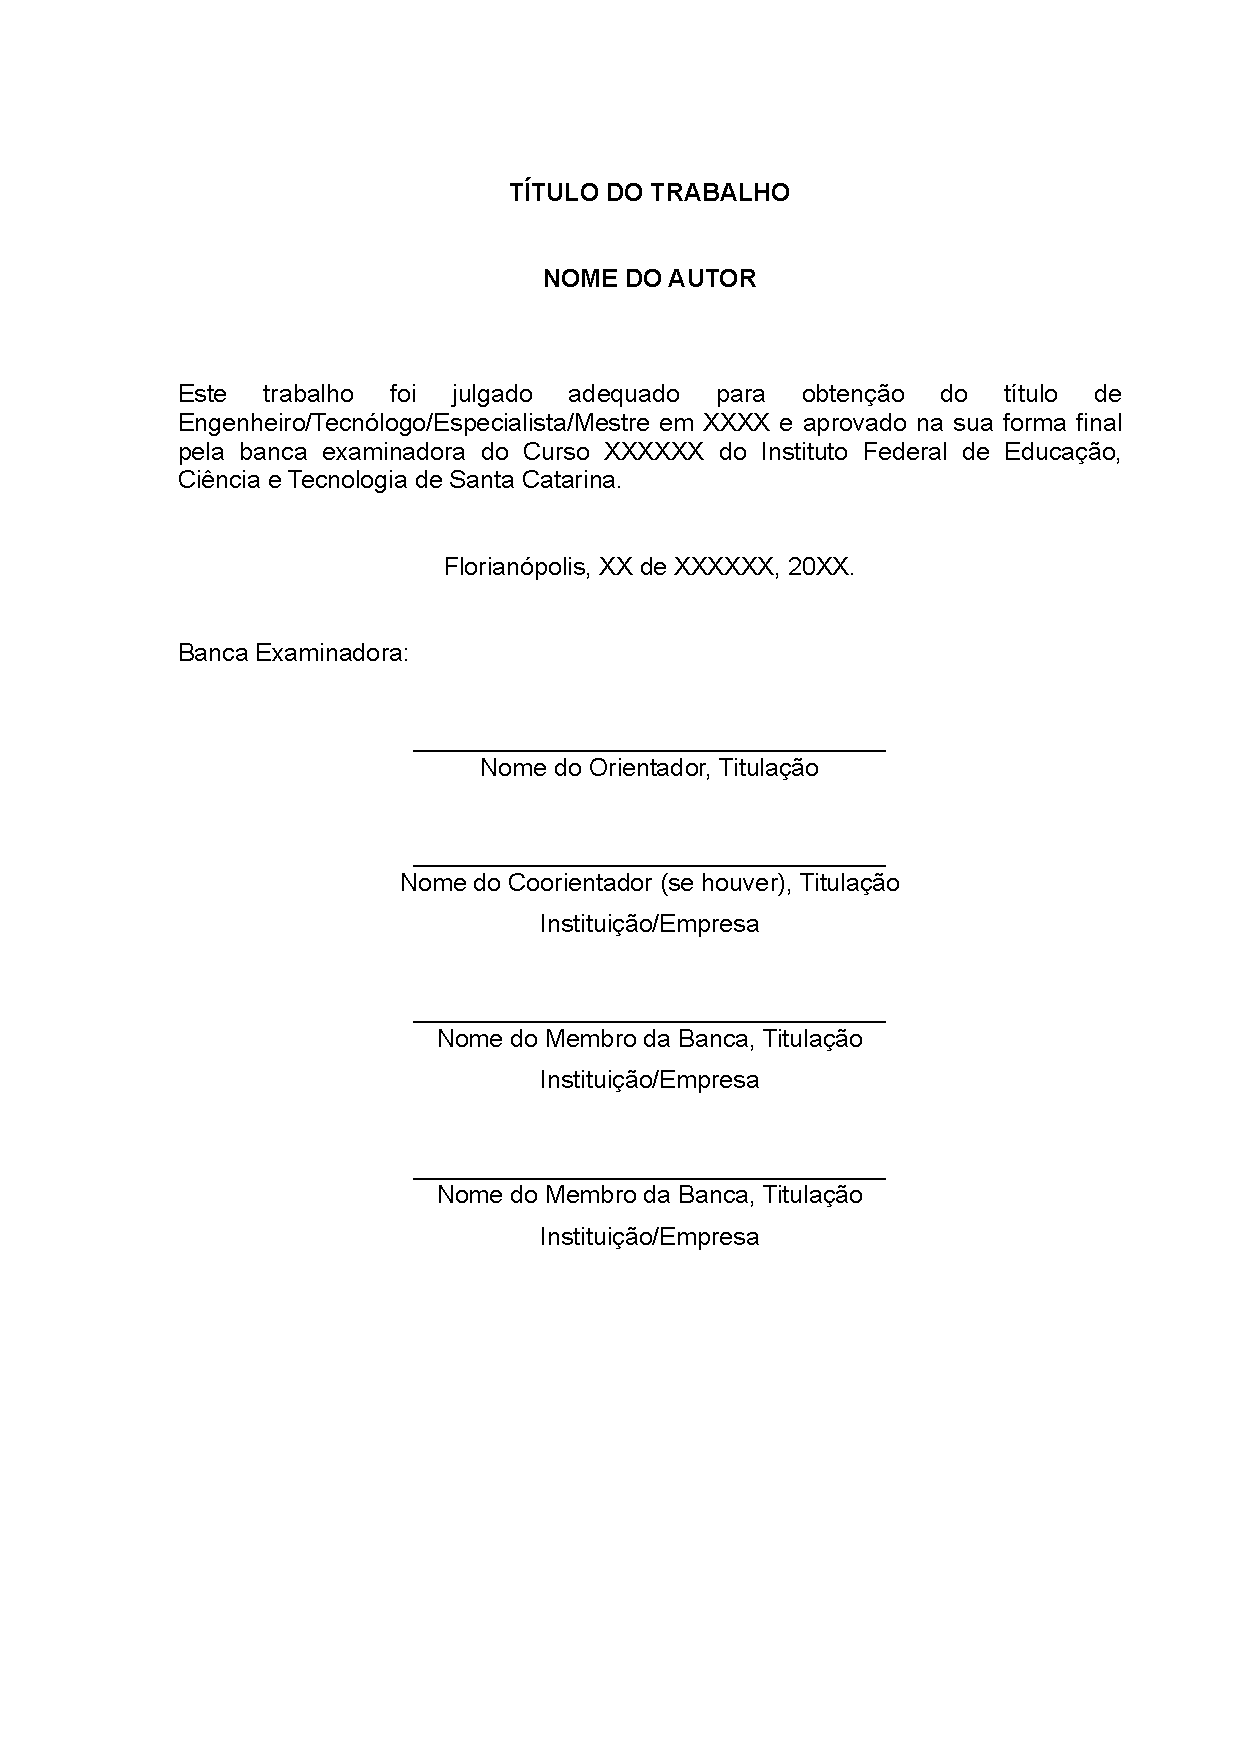
\includepdf[pages=-]{pdf/tcc-aprovado.pdf}

%\cleardoublepage

%---------------------------------------------------------------------%
% Dedicatória
%---------------------------------------------------------------------%
\begin{dedicatoria}
    \vspace*{\fill}
	\begin{flushright}
    		(Dedicatória é um elemento opcional.\\ 
            Texto alinhado no canto inferior direito.\\
            Não deve ultrapassar uma página.)
	\end{flushright}
\end{dedicatoria}




%---------------------------------------------------------------------%
% Agradecimentos
%---------------------------------------------------------------------%
\begin{agradecimentos}
    Elemento opcional que não pode ultrapassar o limite de uma página.
\end{agradecimentos}
% ---

%---------------------------------------------------------------------%
% Epígrafe
%---------------------------------------------------------------------%
\begin{epigrafe}
    \vspace*{\fill}
	\begin{flushright}
    		(Epígrafe é um elemento opcional.\\
    		Texto alinhado no canto inferior direito.\\
            Não deve ultrapassar uma página.)
	\end{flushright}
\end{epigrafe}

%---------------------------------------------------------------------%
% RESUMOS
%---------------------------------------------------------------------%
% resumo em português
\setlength{\absparsep}{18pt} % ajusta o espaçamento dos parágrafos do resumo
\renewcommand{\baselinestretch}{1} 
\begin{resumo}
    O resumo deve mostrar a natureza e o objetivo do trabalho, o método que foi empregado, os resultados e as conclusões. O resumo deve conter entre 150 e 500 palavras e constitui-se de um único parágrafo, sem recuo.

 
   \noindent 
    \textbf{Palavras-chave}: Primeira palavra-chave. Segunda palavra-chave. Terceira palavra-chave. Quarta palavra-chave (opcional). Quinta palavra-chave (opcional). 
\end{resumo}

% resumo em inglês
\renewcommand{\baselinestretch}{1} 
\begin{resumo}[Abstract]
 \begin{otherlanguage*}{english}

   The abstract should show the nature and scope of work, the method that was used, the results and conclusions. The abstract may contain between 150 and 500 words, and it must be only one paragraph. 


   %\vspace{-0.8cm}
 
   \noindent 
   \textbf{Keywords}: First keyword. Second keyword. Third keyword. Fourth keyword (optional). Fifth keyword (optional).  
 \end{otherlanguage*}
\end{resumo}


%---------------------------------------------------------------------%
% inserir lista de ilustrações
%---------------------------------------------------------------------%
\renewcommand{\listfigurename}{Lista de Figuras}
\pdfbookmark[0]{\listfigurename}{lof}
\listoffigures*
\cleardoublepage

%---------------------------------------------------------------------%
% inserir lista de quadros
%---------------------------------------------------------------------%

\renewcommand{\listquadroname}{Lista de quadros}
\newfloat{quadro}{\quadroname}{loq}[chapter]
\setfloatlocations{quadro}{hbtp}
\newlistof{listofquadros}{loq}{\listquadroname}
\newlistentry{quadro}{loq}{0}
\renewcommand{\cftquadroname}{\quadroname\space}
\renewcommand*{\cftquadroaftersnum}{\hfill\textendash\hfill}
\counterwithout{quadro}{chapter}
\listofquadros* 
\cleardoublepage



%---------------------------------------------------------------------%
% inserir lista de tabelas
%---------------------------------------------------------------------%
\pdfbookmark[0]{\listtablename}{lot}
\listoftables*
\cleardoublepage

%---------------------------------------------------------------------%
% inserir lista de listings
%---------------------------------------------------------------------%
%\pdfbookmark[0]{\lstlistlistingname}{lol}
%\listoflistings
%\cleardoublepage

%---------------------------------------------------------------------%
% inserir lista de abreviaturas e simbolos
%---------------------------------------------------------------------%
%\listofabrev{tex/00-Abreviaturas}
\imprimirlistadeabreviaturas

% \imprimirlistadesimbolos
\cleardoublepage

%---------------------------------------------------------------------%
% inserir o sumario

%---------------------------------------------------------------------%


\setlength{\cftbeforechapterskip}{4pt plus 0pt}
\pdfbookmark[0]{\contentsname}{toc}
\tableofcontents*
\cleardoublepage

% ----------------------------------------------------------
% ELEMENTOS TEXTUAIS
% ----------------------------------------------------------
\textual
\pagestyle{parpage}%
\aliaspagestyle{chapter}{parpage}
% ----------------------------------------------------------
% Inclusão dos capítulos que estão em outros arquivos .tex
% ----------------------------------------------------------

\chapter{Introdução}


Texto texto texto texto texto texto texto texto texto texto texto texto texto texto texto texto texto texto texto texto texto texto texto texto texto texto texto texto texto texto texto texto texto texto texto texto texto texto texto. 
\abreviatura{IFSC}{Instituto Federal de Santa Catarina}
\abreviatura{LER}{Lesão por Esforço Repetitivo} 
\abreviatura{IoT}{\textit{Internet of Things} (Internet das Coisas)}
\abreviatura{ANEEL}{Agência Nacional de Energia Elétrica}
\abreviatura{IBM}{\textit{International Business Machines}}


\section{Justificativa}

Texto texto texto texto texto texto texto texto texto texto texto texto texto texto texto texto texto texto texto texto texto texto texto texto texto texto texto texto texto texto texto texto texto texto texto texto texto texto texto \citep{ref:Ellis2021}.

\section{Definição do Problema}

Texto texto texto texto texto texto texto texto texto texto texto texto texto texto texto texto texto texto texto texto texto texto texto texto texto texto texto texto texto texto texto texto texto texto texto texto texto texto texto \citep{ref:vazquez}.

\section{Objetivos}

\subsection{Objetivo Geral}

Texto texto texto texto texto texto texto texto texto texto texto texto texto texto texto texto texto texto texto texto texto texto texto texto texto texto texto texto texto texto texto texto texto texto texto texto texto texto texto.

\subsection{Objetivos Específicos}

Texto texto texto texto:
\begin{alineas}
    \item texto texto texto texto texto texto texto texto texto texto texto texto texto texto texto texto texto texto texto texto texto texto texto texto texto texto texto texto texto texto texto texto texto texto texto texto texto texto;
    \item texto texto texto texto texto texto texto texto texto texto texto texto texto texto texto texto texto texto texto texto texto texto texto texto texto texto texto texto texto texto texto texto texto texto texto texto texto texto; 
    \item texto texto texto texto texto texto texto texto texto texto texto texto texto texto texto texto texto texto texto texto texto texto texto texto texto texto texto texto texto texto texto texto texto texto texto texto texto texto.
\end{alineas}
    
\section{Estrutura do Trabalho}

Texto texto texto texto texto texto texto texto texto texto texto texto texto texto texto texto texto texto texto texto texto texto. 

\chapter{Fundamentação Teórica}

Texto texto texto texto texto texto texto texto texto texto texto texto texto texto texto texto texto texto texto texto texto texto texto texto texto texto texto texto texto texto texto texto texto texto texto texto texto texto texto.

\section{Subtítulo Secundário 1}

Texto texto texto texto texto texto texto texto texto texto texto texto texto texto texto texto texto texto texto texto texto texto texto texto texto texto texto texto texto texto texto texto texto texto texto texto texto texto texto, conforme descrito por \citet{pressman} e como mostra o Quadro \ref{quadro1}.


\begin{quadro}[h]
\centering

\caption{Tipos de energia analisados}
\begin{tabular}{|c|c|}
\hline
\textbf{Ano} & \textbf{Tipos de energia} \\ \hline
2017         & Mecânica                  \\ \hline
2018         & Térmica                   \\ \hline
2019         & Elétrica                  \\ \hline
2020         & Química                   \\ \hline
2021         & Atômica                   \\ \hline
\end{tabular}
\label{quadro1}
\\
\small{Fonte: Elaboração própria (2021).} 
\end{quadro}

\section{Subtítulo Secundário 2}

As citações diretas com menos de três linhas “devem estar entre aspas e devem mostrar entre parênteses o ano e a página da obra consultada.” (AUTOR, ano, página). Já as citações com mais de três linhas devem ser recuadas da margem esquerda em 4 cm, tamanho da fonte 10, espaçamento simples e texto sem aspas (ABNT, 2002, p. 2).



 \begin{citacao}
            \begin{alineas}[leftmargin=\leftskip+\labelwidth-\labelsep]
                Texto texto texto texto texto texto texto texto. Texto texto texto texto texto texto. Texto texto texto texto texto texto texto texto texto. Texto texto texto texto texto texto Texto texto texto texto texto texto. Texto texto texto texto texto texto. (\citeauthor{ref:ibmm}, \citeyear{ref:ibmm}, p. 20).
            \end{alineas}
\end{citacao}



\subsection{Subtítulo Terciário}

Texto texto texto texto texto texto texto texto texto texto texto texto texto texto texto texto texto texto texto texto texto texto texto texto texto texto texto texto texto texto texto texto texto.


\subsubsection{Subtítulo Quaternário}

Texto texto texto texto texto texto texto texto texto texto texto texto texto texto texto texto texto texto texto texto texto texto texto texto texto texto texto texto texto texto texto texto texto  (conforme exposto na Figura \ref{fig:motor}).



    \begin{figure}[H]
    	\centering
    	\caption{Motor Weg W22}
    	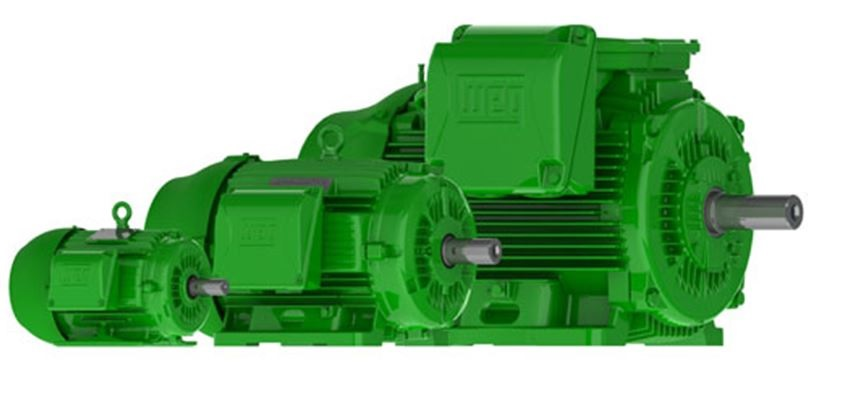
\includegraphics[scale=0.45]{figuras/motor.jpg}
    	\label{fig:motor}
    	\\
        \vspace{-0.8cm}\hspace{-7cm}\small{Fonte: WEG (2014).} 
    \end{figure}
    
    Texto texto texto texto texto texto texto texto texto texto texto texto texto texto texto conforme indica a Tabela \ref{tabela1}.

    

\begin{table}[h]
\centering
\caption{Produção de petróleo na Bahia}
\begin{tabular}{ c c }
\ChangeRT{2pt}
Ano  & Produção (1000 t) \\ \ChangeRT{2pt}
1996 & 2.536             \\ 
1997 & 2.665             \\ 
1998 & 3.056             \\ 
1999 & 3.567             \\ 
2021 & Atômica           \\ \ChangeRT{2pt}
\end{tabular}
\label{tabela1}
\\
\small{Fonte: Adaptado de ANP (2000).}    
\end{table}



    
    Texto texto texto texto texto texto texto texto texto texto texto texto texto texto texto texto texto texto texto texto texto texto texto texto texto texto texto texto texto texto texto texto texto 
    Texto texto texto texto texto texto texto texto texto texto texto texto texto texto texto texto texto texto texto texto texto texto texto texto texto texto texto texto texto texto texto texto texto como evidencia a Figura  \ref{fig:diagrama}.
    
    
    
    \begin{figure}[H]
    	\centering
    	\caption{Diagrama Fasorial}
    	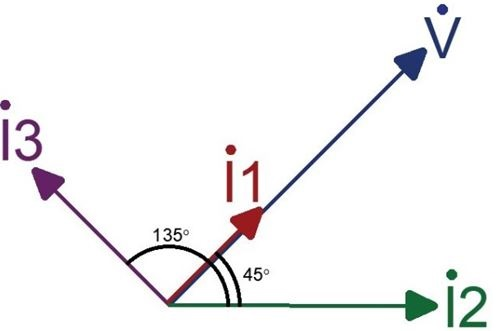
\includegraphics[scale=0.45]{figuras/diagrama.jpg}
    	\label{fig:diagrama}
    	\\
    	\vspace{0.2cm}\hspace{-3cm}\small{Fonte: Silva (2020).}
    \end{figure}
    
    Texto texto texto texto texto texto texto texto texto texto texto texto texto texto texto texto texto texto texto texto texto texto texto texto texto texto texto texto texto texto texto texto, conforme mostra a Equação \ref{eq:baskara}.
    
\begin{equation} \label{eq:baskara}
  x=\frac{-b\pm\sqrt{b^2-4ac}}{2a}
\end{equation} 

\chapter{Metodologia}

Texto texto texto texto texto texto texto texto texto texto texto texto texto texto texto texto texto texto texto texto texto texto texto texto texto texto texto texto texto texto texto texto texto texto texto texto texto texto texto \citep{ref:Fensel,ref:booch}.




\section{Métodos Aplicados}

Texto texto texto texto texto texto texto texto texto texto texto texto texto texto texto texto texto texto texto texto texto texto texto texto texto texto texto texto texto texto texto texto texto texto texto texto texto texto texto.

\chapter{Apresentação dos Resultados}

Texto texto texto texto texto texto texto texto texto texto texto texto texto texto texto texto texto texto texto texto texto texto texto texto texto texto texto texto texto texto texto texto texto texto texto texto texto texto texto.

\section{Análise e discussão dos resultados}

Texto texto texto texto texto texto texto texto texto texto texto texto texto texto texto texto texto texto texto texto texto texto texto texto texto texto texto texto texto texto texto texto texto texto texto texto texto texto texto.

\chapter{Considerações Finais}

Texto texto texto texto texto texto texto texto texto texto texto texto texto texto texto texto texto texto texto texto texto texto texto texto texto texto texto texto texto texto texto texto texto texto texto texto texto texto texto.

\section{Sugestões para trabalhos futuros}

Texto texto texto texto texto texto texto texto texto texto texto texto texto texto texto texto texto texto texto texto texto texto texto texto texto texto texto texto texto texto texto texto texto texto texto texto texto texto texto.

\chapter{Futuros trabalhos}

Texto texto texto texto texto texto texto texto texto texto texto texto texto texto texto texto texto texto texto texto texto texto texto texto texto texto texto texto texto texto texto texto texto texto texto texto texto texto texto.

\section{Sugestões para trabalhos futuros}

Texto texto texto texto texto texto texto texto texto texto texto texto texto texto texto texto texto texto texto texto texto texto texto texto texto texto texto texto texto texto texto texto texto texto texto texto texto texto texto.


% ----------------------------------------------------------
% Como realizar a citação bibliográfica
% ----------------------------------------------------------

%\citet{jon90} = Jones et al. (1990)
%\citet[chap.~2]{jon90} = Jones et al. (1990, chap. 2)
%\citep{jon90} = (Jones et al., 1990)
%\citep[chap.~2]{jon90} = (Jones et al., 1990, chap. 2)
%%\citep[see][]{jon90} = (see Jones et al., 1990)
%\citep[see][chap.~2]{jon90} = (see Jones et al., 1990, chap. 2)
%\citet*{jon90} = Jones, Baker, and Williams (1990)
%\citep*{jon90} = (Jones, Baker, and Williams, 1990)



% ----------------------------------------------------------
% ELEMENTOS PÓS-TEXTUAIS
% ----------------------------------------------------------
\postextual
% ----------------------------------------------------------

% ----------------------------------------------------------
% Referências bibliográficas
% ----------------------------------------------------------
\bibliography{referencias}
\bibliographystyle{apalike-ejor}

% ----------------------------------------------------------
% Apêndices
% ----------------------------------------------------------
 \begin{apendicesenv}         
     \partapendices
     \chapter{Apêndices}

\chapter{Título}

\begin{longtable}[htbp]{llcrr}
\label{tab:primeiros_focos}

\caption{Primeiros registros de focos de \textit{Aedes} sp. em municípios catarinenses.} \\
\hline
\rowcolor{darkgray} \textcolor{white}{Semana} & \textcolor{white}{Município} & \textcolor{white}{Focos} & \textcolor{white}{Latitude} & \textcolor{white}{Longitude} \\
\hline
\endfirsthead

\caption{(Continuação) Primeiros registros de focos de \textit{Aedes} sp. em municípios catarinenses.} \\
\rowcolor{darkgray} \textcolor{white}{Semana} & \textcolor{white}{Município} & \textcolor{white}{Focos} & \textcolor{white}{Latitude} & \textcolor{white}{Longitude} \\
\hline
\endhead

\hline
\textit{Continua na próxima página}
\hline 
\endfoot

\hline
\textit{Finalização da tabela} \\
\hline
\endlastfoot

2012-01-01 & BALNEÁRIO CAMBORIÚ & 2 & -27.004737 & -48.621741 \\
2012-01-01 & BLUMENAU & 1 & -26.885767 & -49.097309 \\
2012-01-01 & BOMBINHAS & 2 & -27.173256 & -48.517487 \\
2012-01-01 & CHAPECÓ & 1 & -27.125144 & -52.650339 \\
2012-01-01 & FLORIANÓPOLIS & 1 & -27.577834 & -48.508198 \\
2012-01-01 & SÃO MIGUEL DO OESTE & 3 & -26.727237 & -53.512121 \\
2012-01-01 & TIJUCAS & 2 & -27.247563 & -48.700886 \\
2012-01-01 & XANXERÊ & 1 & -26.872279 & -52.409754 \\
2012-01-08 & JOINVILLE & 1 & -26.244282 & -48.951405 \\
2012-01-15 & ARAQUARI & 2 & -26.461708 & -48.757777 \\
2012-01-15 & BRUSQUE & 1 & -27.125000 & -48.909743 \\
2012-01-15 & GUARAMIRIM & 1 & -26.476551 & -48.944882 \\
2012-01-22 & DIONÍSIO CERQUEIRA & 1 & -26.329843 & -53.533105 \\
2012-01-29 & BIGUAÇU & 1 & -27.433530 & -48.693947 \\
2012-01-29 & JARAGUÁ DO SUL & 1 & -26.481908 & -49.159974 \\
2012-01-29 & SAUDADES & 1 & -26.897207 & -53.040014 \\
2012-01-29 & SÃO JOSÉ & 1 & -27.578471 & -48.656256 \\
2012-02-05 & SÃO JOÃO DO OESTE & 1 & -27.091607 & -53.591664 \\
2012-02-12 & JAGUARUNA & 2 & -28.657896 & -49.044748 \\
2012-02-12 & SÃO JOSÉ DO CEDRO & 3 & -26.480851 & -53.533736 \\
2012-02-19 & ITAPOÁ & 1 & -26.082477 & -48.652354 \\
2012-02-26 & BARRA VELHA & 1 & -26.662441 & -48.727386 \\
2012-02-26 & CRICIÚMA & 1 & -28.715695 & -49.379716 \\
2012-02-26 & MASSARANDUBA & 1 & -26.626911 & -48.988192 \\
2012-02-26 & PALMITOS & 1 & -27.092622 & -53.179829 \\
2012-03-04 & ARARANGUÁ & 1 & -28.942293 & -49.471174 \\
2012-03-04 & GAROPABA & 1 & -28.046734 & -48.658936 \\
2012-03-04 & PALHOÇA & 1 & -27.771821 & -48.661708 \\
2012-03-04 & PAULO LOPES & 1 & -27.964855 & -48.760163 \\
2012-03-11 & BENEDITO NOVO & 1 & -26.800940 & -49.435396 \\
2012-03-11 & CAPIVARI DE BAIXO & 2 & -28.455564 & -48.943385 \\
2012-03-11 & CONCÓRDIA & 5 & -27.239127 & -52.007382 \\
2012-03-11 & PORTO UNIÃO & 1 & -26.383628 & -51.007785 \\
2012-03-11 & RIO DO SUL & 1 & -27.196051 & -49.629953 \\
2012-03-11 & SIDERÓPOLIS & 1 & -28.583272 & -49.526696 \\
2012-03-11 & SOMBRIO & 1 & -29.070191 & -49.655927 \\
2012-03-18 & LAURENTINO & 1 & -27.207982 & -49.733614 \\
2012-03-25 & APIÚNA & 1 & -27.124502 & -49.364245 \\
2012-03-25 & CANOINHAS & 1 & -26.249950 & -50.533371 \\
2012-03-25 & SÃO FRANCISCO DO SUL & 2 & -26.261597 & -48.640319 \\
2012-03-25 & TUBARÃO & 1 & -28.481581 & -49.037249 \\
2012-04-01 & NAVEGANTES & 1 & -26.828743 & -48.727396 \\
2012-04-01 & PINHALZINHO & 14 & -26.829373 & -52.976632 \\
2012-04-15 & PIRATUBA & 1 & -27.461219 & -51.772820 \\
2012-04-22 & GARUVA & 1 & -26.057112 & -48.867328 \\
2012-04-22 & POMERODE & 1 & -26.728186 & -49.173304 \\
2012-05-06 & XAXIM & 1 & -26.970309 & -52.529105 \\
2012-05-20 & PORTO BELO & 1 & -27.174796 & -48.616435 \\
2012-05-20 & SÃO BENTO DO SUL & 1 & -26.294902 & -49.349982 \\
2012-05-27 & GASPAR & 1 & -26.931343 & -48.966033 \\
2012-06-10 & COCAL DO SUL & 1 & -28.598697 & -49.333930 \\
2012-06-10 & ITAPIRANGA & 1 & -27.112222 & -53.711674 \\
2012-07-15 & SÃO LOURENÇO DO OESTE & 1 & -26.465488 & -52.859773 \\
2012-08-12 & CAMPO ALEGRE & 1 & -26.120556 & -49.217539 \\
2012-09-02 & CAIBI & 1 & -27.025176 & -53.263058 \\
2012-09-02 & MARAVILHA & 1 & -26.759974 & -53.198113 \\
2012-09-16 & BRAÇO DO NORTE & 1 & -28.240945 & -49.142365 \\
2012-10-07 & INDAIAL & 1 & -26.994979 & -49.224178 \\
2012-10-07 & ITAPEMA & 1 & -27.108583 & -48.634427 \\
2012-10-28 & LAGES & 1 & -28.020467 & -50.340573 \\
2012-11-18 & IMBITUBA & 1 & -28.194274 & -48.702663 \\
2012-12-23 & SÃO DOMINGOS & 1 & -26.539387 & -52.554602 \\
2012-12-30 & GUATAMBÚ & 10 & -27.116474 & -52.783390 \\
2013-01-20 & BALNEÁRIO PIÇARRAS & 13 & -26.759492 & -48.733290 \\
2013-01-20 & CORONEL FREITAS & 3 & -26.883161 & -52.725052 \\
2013-01-20 & LAGUNA & 1 & -28.486421 & -48.825930 \\
2013-01-27 & CORDILHEIRA ALTA & 1 & -26.975707 & -52.641660 \\
2013-01-27 & ITAJAÍ & 1 & -26.969013 & -48.753417 \\
2013-02-10 & RIQUEZA & 1 & -26.978455 & -53.344352 \\
2013-02-24 & PRINCESA & 1 & -26.432945 & -53.611776 \\
2013-02-24 & SANTA ROSA DO SUL & 2 & -29.121483 & -49.743751 \\
2013-03-03 & BELMONTE & 1 & -26.857082 & -53.618060 \\
2013-03-03 & CAÇADOR & 1 & -26.763016 & -51.084665 \\
2013-03-17 & ITUPORANGA & 1 & -27.453450 & -49.538870 \\
2013-03-17 & SANTO AMARO DA IMPERATRIZ & 3 & -27.741766 & -48.796550 \\
2013-04-14 & IMARUÍ & 1 & -28.231479 & -48.834413 \\
2013-04-14 & MONDAÍ & 1 & -27.099293 & -53.446497 \\
2013-04-14 & NOVA ERECHIM & 1 & -26.908169 & -52.906693 \\
2013-05-05 & ÁGUAS DE CHAPECÓ & 1 & -27.054386 & -52.956735 \\
2013-05-19 & ANTÔNIO CARLOS & 1 & -27.497474 & -48.830982 \\
2013-05-26 & QUILOMBO & 1 & -26.729236 & -52.717982 \\
2013-06-02 & GUARACIABA & 1 & -26.580106 & -53.571076 \\
2013-06-02 & IRANI & 1 & -27.025235 & -51.917948 \\
2013-06-02 & VIDEIRA & 1 & -27.006590 & -51.126791 \\
2013-06-16 & SÃO JOÃO BATISTA & 1 & -27.328928 & -48.859016 \\
2013-06-30 & FORMOSA DO SUL & 1 & -26.634189 & -52.793789 \\
2013-06-30 & RIO NEGRINHO & 1 & -26.442714 & -49.596156 \\
2013-06-30 & SÃO LUDGERO & 1 & -28.353135 & -49.168162 \\
2013-07-28 & DESCANSO & 1 & -26.858414 & -53.479301 \\
2013-07-28 & JOAÇABA & 1 & -27.151796 & -51.592935 \\
2013-09-29 & CAMBORIÚ & 1 & -27.070939 & -48.708989 \\
2013-09-29 & CORUPÁ & 1 & -26.439934 & -49.326711 \\
2013-09-29 & MAFRA & 1 & -26.200812 & -49.889559 \\
2013-10-06 & IBIRAMA & 1 & -27.018150 & -49.528544 \\
2013-10-06 & ITÁ & 1 & -27.244015 & -52.332158 \\
2013-10-06 & PARAÍSO & 1 & -26.662800 & -53.678304 \\
2013-11-03 & CAPÃO ALTO & 1 & -28.062182 & -50.606912 \\
2013-11-24 & ORLEANS & 1 & -28.279938 & -49.371860 \\
2013-12-29 & CATANDUVAS & 3 & -27.044998 & -51.696411 \\
2013-12-29 & GUARUJÁ DO SUL & 1 & -26.398336 & -53.484021 \\
2013-12-29 & RIO DO OESTE & 1 & -27.158977 & -49.841673 \\
2014-01-05 & IPUAÇU & 1 & -26.678739 & -52.476014 \\
2014-01-12 & GRAVATAL & 1 & -28.354020 & -49.019524 \\
2014-01-19 & IÇARA & 5 & -28.751615 & -49.277346 \\
2014-02-09 & PENHA & 1 & -26.807760 & -48.650765 \\
2014-02-16 & GOVERNADOR CELSO RAMOS & 1 & -27.376617 & -48.577230 \\
2014-02-16 & PASSO DE TORRES & 1 & -29.267248 & -49.721932 \\
2014-02-16 & TIMBÓ & 1 & -26.808192 & -49.268848 \\
2014-03-02 & SALTINHO & 1 & -26.590522 & -53.022279 \\
2014-03-09 & CAMPO ERÊ & 1 & -26.450419 & -53.130290 \\
2014-03-09 & LUZERNA & 2 & -27.090413 & -51.505633 \\
2014-03-09 & SERRA ALTA & 1 & -26.692621 & -53.025238 \\
2014-03-23 & TREZE TÍLIAS & 1 & -26.964791 & -51.449354 \\
2014-04-06 & CUNHATAÍ & 2 & -26.975087 & -53.100870 \\
2014-04-06 & IRATI & 2 & -26.627592 & -52.890099 \\
2014-04-06 & SUL BRASIL & 2 & -26.695342 & -52.946800 \\
2014-04-13 & NOVA TRENTO & 1 & -27.313268 & -49.041367 \\
2014-04-13 & SÃO CARLOS & 1 & -27.030109 & -53.031412 \\
2014-04-20 & ENTRE RIOS & 1 & -26.739710 & -52.578368 \\
2014-04-20 & SCHROEDER & 1 & -26.367952 & -49.060456 \\
2014-04-27 & VARGEM BONITA & 1 & -26.944996 & -51.756631 \\
2014-05-11 & CUNHA PORÃ & 2 & -26.879228 & -53.190665 \\
2014-05-11 & TRÊS BARRAS & 1 & -26.169921 & -50.255230 \\
2014-05-18 & ÁGUAS MORNAS & 1 & -27.733481 & -48.936027 \\
2014-05-25 & UNIÃO DO OESTE & 3 & -26.786666 & -52.856010 \\
2014-08-10 & CAPINZAL & 2 & -27.411939 & -51.630815 \\
2014-08-10 & FORQUILHINHA & 3 & -28.781693 & -49.493283 \\
2014-08-10 & SÃO JOÃO DO ITAPERIÚ & 1 & -26.591052 & -48.797733 \\
2014-08-10 & TREVISO & 5 & -28.499162 & -49.489841 \\
2014-09-07 & ARVOREDO & 1 & -27.070854 & -52.441987 \\
2014-09-07 & CAXAMBU DO SUL & 1 & -27.146711 & -52.920211 \\
2014-09-07 & IBICARÉ & 1 & -27.092470 & -51.370040 \\
2014-09-07 & OURO & 5 & -27.283437 & -51.681886 \\
2014-10-05 & BOM JESUS & 1 & -26.739042 & -52.389991 \\
2014-10-12 & PLANALTO ALEGRE & 1 & -27.051964 & -52.868983 \\
2014-11-09 & GUABIRUBA & 4 & -27.103338 & -49.020750 \\
2014-12-14 & ARABUTÃ & 1 & -27.140868 & -52.181545 \\
2014-12-14 & BALNEÁRIO BARRA DO SUL & 8 & -26.446419 & -48.652569 \\
2014-12-14 & BALNEÁRIO RINCÃO & 3 & -28.826740 & -49.254237 \\
2014-12-14 & BOTUVERÁ & 3 & -27.218576 & -49.123526 \\
2014-12-14 & ILHOTA & 7 & -26.859041 & -48.857351 \\
2014-12-14 & JARDINÓPOLIS & 1 & -26.717195 & -52.871306 \\
2014-12-14 & LUIZ ALVES & 1 & -26.727352 & -48.891082 \\
2014-12-14 & PERITIBA & 4 & -27.351361 & -51.875059 \\
2014-12-14 & PESCARIA BRAVA & 2 & -28.401764 & -48.883642 \\
2014-12-14 & SEARA & 3 & -27.147833 & -52.340694 \\
2014-12-21 & HERVAL D'OESTE & 10 & -27.195376 & -51.410665 \\
2014-12-21 & IBIAM & 1 & -27.208374 & -51.215463 \\
2014-12-21 & TANGARÁ & 1 & -27.147028 & -51.147069 \\
2014-12-28 & SANTA TEREZINHA DO PROGRESSO & 2 & -26.592749 & -53.169925 \\
2015-01-04 & ANCHIETA & 1 & -26.532948 & -53.333109 \\
2015-01-04 & NOVA ITABERABA & 3 & -26.961142 & -52.833166 \\
2015-01-04 & SÃO BERNARDINO & 1 & -26.487695 & -52.987611 \\
2015-01-11 & ARMAZÉM & 1 & -28.237881 & -49.014678 \\
2015-01-18 & CAMPOS NOVOS & 1 & -27.413002 & -51.244612 \\
2015-01-25 & CORONEL MARTINS & 1 & -26.534646 & -52.671875 \\
2015-02-01 & ABELARDO LUZ & 1 & -26.562427 & -52.255719 \\
2015-02-08 & JUPIÁ & 1 & -26.394106 & -52.720920 \\
2015-02-15 & XAVANTINA & 1 & -27.021214 & -52.321890 \\
2015-03-01 & PALMA SOLA & 1 & -26.373544 & -53.314529 \\
2015-03-29 & LONTRAS & 1 & -27.189434 & -49.507309 \\
2015-04-12 & BOM JESUS DO OESTE & 2 & -26.684021 & -53.095288 \\
2015-04-12 & NOVO HORIZONTE & 2 & -26.494979 & -52.796361 \\
2015-04-19 & NOVA VENEZA & 1 & -28.684718 & -49.584912 \\
2015-04-26 & GALVÃO & 2 & -26.449409 & -52.659011 \\
2015-04-26 & SÃO MARTINHO & 1 & -28.124557 & -48.971904 \\
2015-05-03 & FLOR DO SERTÃO & 1 & -26.763781 & -53.337342 \\
2015-05-10 & SÃO PEDRO DE ALCÂNTARA & 1 & -27.591567 & -48.837131 \\
2015-05-31 & IRINEÓPOLIS & 1 & -26.357066 & -50.760691 \\
2015-12-13 & MODELO & 2 & -26.774777 & -53.051096 \\
2016-01-03 & IPUMIRIM & 1 & -27.040309 & -52.152891 \\
2016-01-03 & PASSOS MAIA & 1 & -26.706083 & -51.961063 \\
2016-01-17 & RIO DOS CEDROS & 1 & -26.617927 & -49.368385 \\
2016-01-24 & SANGÃO & 1 & -28.651315 & -49.125834 \\
2016-02-14 & IRACEMINHA & 1 & -26.845317 & -53.324456 \\
2016-02-14 & OURO VERDE & 1 & -26.711533 & -52.278758 \\
2016-02-21 & TUNÁPOLIS & 1 & -26.988117 & -53.649949 \\
2016-03-13 & BANDEIRANTE & 1 & -26.768596 & -53.648168 \\
2016-03-13 & CORREIA PINTO & 3 & -27.596830 & -50.378096 \\
2016-03-13 & SÃO MIGUEL DA BOA VISTA & 2 & -26.689643 & -53.239962 \\
2016-03-20 & ROMELÂNDIA & 1 & -26.648390 & -53.317124 \\
2016-03-20 & ÁGUA DOCE & 1 & -26.764469 & -51.612406 \\
2016-04-10 & CURITIBANOS & 1 & -27.292934 & -50.617548 \\
2016-05-08 & PRESIDENTE GETÚLIO & 1 & -27.062584 & -49.714430 \\
2016-06-05 & MORRO DA FUMAÇA & 1 & -28.637696 & -49.242862 \\
2016-10-02 & TURVO & 1 & -28.903082 & -49.703422 \\
2016-10-30 & ASCURRA & 1 & -26.973634 & -49.395966 \\
2016-11-06 & AGROLÂNDIA & 1 & -27.455116 & -49.824780 \\
2016-11-20 & MARACAJÁ & 1 & -28.863963 & -49.455547 \\
2016-11-27 & FRAIBURGO & 1 & -27.037815 & -50.872432 \\
2016-11-27 & SALETE & 1 & -26.969623 & -50.010685 \\
2016-12-18 & ÁGUAS FRIAS & 1 & -26.851639 & -52.852311 \\
2017-01-01 & MELEIRO & 1 & -28.841751 & -49.601794 \\
2017-03-05 & PAINEL & 1 & -27.963630 & -50.072135 \\
2017-03-12 & TIGRINHOS & 1 & -26.676067 & -53.156546 \\
2017-03-19 & IPORÃ DO OESTE & 5 & -27.000432 & -53.489414 \\
2017-04-16 & AGRONÔMICA & 1 & -27.327559 & -49.720747 \\
2017-04-30 & SANTIAGO DO SUL & 1 & -26.630874 & -52.697312 \\
2017-05-21 & LAJEADO GRANDE & 1 & -26.854941 & -52.552085 \\
2017-06-18 & SÃO JOÃO DO SUL & 1 & -29.205567 & -49.813468 \\
2017-07-09 & ALTO BELA VISTA & 1 & -27.421535 & -51.925948 \\
2017-07-30 & MONTE CASTELO & 1 & -26.660694 & -50.291540 \\
2017-07-30 & VARGEÃO & 1 & -26.778693 & -52.124176 \\
2017-12-31 & FAXINAL DOS GUEDES & 3 & -26.846669 & -52.244323 \\
2018-01-07 & BALNEÁRIO GAIVOTA & 1 & -29.153516 & -49.615368 \\
2018-01-21 & LINDÓIA DO SUL & 1 & -27.031507 & -52.052466 \\
2018-01-28 & BARRA BONITA & 1 & -26.668358 & -53.425055 \\
2018-03-25 & BALNEÁRIO ARROIO DO SILVA & 1 & -29.019465 & -49.475057 \\
2018-03-25 & GRÃO-PARÁ & 1 & -28.155035 & -49.314022 \\
2018-05-13 & PONTE SERRADA & 6 & -26.861769 & -51.928214 \\
2018-06-10 & JACINTO MACHADO & 1 & -28.994832 & -49.848148 \\
2018-07-01 & PAIAL & 1 & -27.213003 & -52.487869 \\
2018-11-11 & LACERDÓPOLIS & 1 & -27.250882 & -51.590311 \\
2019-01-06 & MAREMA & 3 & -26.812383 & -52.630070 \\
2019-01-13 & LAURO MÜLLER & 1 & -28.384585 & -49.451932 \\
2019-01-13 & PONTE ALTA DO NORTE & 2 & -27.180289 & -50.418567 \\
2019-01-13 & SANTA HELENA & 3 & -26.921956 & -53.619652 \\
2019-01-20 & SÃO CRISTÓVÃO DO SUL & 1 & -27.295206 & -50.349497 \\
2019-01-20 & WITMARSUM & 1 & -26.937345 & -49.841761 \\
2019-02-10 & POUSO REDONDO & 1 & -27.286166 & -49.977272 \\
2019-02-10 & SALTO VELOSO & 1 & -26.895935 & -51.428018 \\
2019-02-17 & IPIRA & 1 & -27.370819 & -51.798708 \\
2019-03-03 & TAIÓ & 1 & -27.078456 & -50.092435 \\
2019-03-24 & PAPANDUVA & 3 & -26.502424 & -50.172362 \\
2019-06-30 & BRAÇO DO TROMBUDO & 1 & -27.368599 & -49.903617 \\
2019-10-20 & PRAIA GRANDE & 1 & -29.181868 & -49.989502 \\
2019-11-24 & URUSSANGA & 1 & -28.492699 & -49.328277 \\
2020-01-26 & PETROLÂNDIA & 1 & -27.545741 & -49.682724 \\
2020-02-09 & ZORTÉA & 1 & -27.476988 & -51.535615 \\
2020-02-16 & RODEIO & 1 & -26.895097 & -49.351036 \\
2020-03-15 & AURORA & 1 & -27.329632 & -49.590347 \\
2020-04-12 & JOSÉ BOITEUX & 1 & -26.859487 & -49.646306 \\
2020-04-19 & CANELINHA & 1 & -27.234604 & -48.802310 \\
2020-04-26 & TROMBUDO CENTRAL & 1 & -27.312097 & -49.811416 \\
2020-05-03 & ANGELINA & 1 & -27.543006 & -49.067224 \\
2020-05-03 & MACIEIRA & 1 & -26.803514 & -51.353132 \\
2020-05-03 & SÃO BONIFÁCIO & 1 & -27.956554 & -48.939098 \\
2020-06-14 & MAJOR GERCINO & 1 & -27.427926 & -49.052632 \\
2020-08-16 & TREZE DE MAIO & 1 & -28.566224 & -49.154191 \\
2021-01-03 & JABORÁ & 1 & -27.141510 & -51.772667 \\
2021-01-10 & ATALANTA & 1 & -27.437304 & -49.742550 \\
2021-01-10 & ERVAL VELHO & 1 & -27.284351 & -51.421890 \\
2021-01-10 & PRESIDENTE NEREU & 1 & -27.268253 & -49.354952 \\
2021-01-17 & ERMO & 1 & -28.990337 & -49.652921 \\
2021-01-24 & ITAIÓPOLIS & 1 & -26.472148 & -49.891245 \\
2021-02-21 & RIO DAS ANTAS & 1 & -26.909076 & -51.063409 \\
2021-02-28 & RIO DO CAMPO & 1 & -26.892307 & -50.131394 \\
2021-03-14 & LEBON RÉGIS & 1 & -26.858429 & -50.702569 \\
2021-03-14 & MAJOR VIEIRA & 2 & -26.481213 & -50.361577 \\
2021-05-09 & CELSO RAMOS & 1 & -27.651969 & -51.308241 \\
2021-08-08 & ARROIO TRINTA & 1 & -26.921499 & -51.336678 \\
2021-09-12 & VIDAL RAMOS & 1 & -27.387882 & -49.347753 \\
2021-10-31 & MORRO GRANDE & 1 & -28.722065 & -49.740484 \\
2021-11-28 & MIRIM DOCE & 1 & -27.185593 & -50.175136 \\
2022-01-09 & IOMERÊ & 5 & -26.987730 & -51.275507 \\
2022-01-16 & DONA EMMA & 1 & -26.988701 & -49.778082 \\
2022-01-23 & PINHEIRO PRETO & 1 & -27.049431 & -51.236054 \\
2022-01-30 & DOUTOR PEDRINHO & 1 & -26.705567 & -49.553839 \\
2022-02-27 & SÃO JOSÉ DO CERRITO & 1 & -27.598272 & -50.650263 \\
2022-03-13 & BOCAINA DO SUL & 1 & -27.763118 & -49.909163 \\
2022-03-13 & IMBUIA & 2 & -27.502913 & -49.406526 \\
2022-03-13 & PRESIDENTE CASTELLO BRANCO & 2 & -27.233335 & -51.780936 \\
2022-03-20 & BOM RETIRO & 1 & -27.785360 & -49.563009 \\
2022-07-31 & MATOS COSTA & 1 & -26.481288 & -51.141830 \\
2023-02-26 & SANTA TEREZINHA & 1 & -26.667603 & -50.005296 \\
2023-03-19 & ANITÁPOLIS & 1 & -27.879776 & -49.138750 \\
2023-03-26 & SANTA CECÍLIA & 1 & -26.926038 & -50.446240 \\
2023-05-14 & ABDON BATISTA & 5 & -27.583825 & -51.056263 \\
2023-11-12 & PEDRAS GRANDES & 1 & -28.479421 & -49.204475 \\
\end{longtable}


\begin{longtable}[htbp]{llcrr}
\label{tab:primeiros_casos}

\caption{Primeiros registros de casos de dengue em municípios catarinenses.} \\
\hline
\rowcolor{darkgray} \textcolor{white}{Semana} & \textcolor{white}{Município} & \textcolor{white}{Casos} & \textcolor{white}{latitude} & \textcolor{white}{longitude} \\
\hline
\endfirsthead

\caption{(Continuação) Primeiros registros de casos de dengue em municípios catarinenses.} \\
\rowcolor{darkgray} \textcolor{white}{Semana} & \textcolor{white}{Município} & \textcolor{white}{Casos} & \textcolor{white}{latitude} & \textcolor{white}{longitude} \\
\hline
\endhead

\hline
\textit{Continua na próxima página}
\hline
\endfoot

\hline
\textit{Finalização da tabela} \\
\hline
\endlastfoot




2014-04-13 & RIO DO SUL & 1 & -27.196051 & -49.629953 \\
2014-05-18 & MORRO DA FUMAÇA & 1 & -28.637696 & -49.242862 \\
2014-06-01 & MASSARANDUBA & 1 & -26.626911 & -48.988192 \\
2014-07-06 & ITAJAÍ & 1 & -26.969013 & -48.753417 \\
2014-12-21 & MARAVILHA & 1 & -26.759974 & -53.198113 \\
2015-02-15 & BLUMENAU & 1 & -26.885767 & -49.097309 \\
2015-03-01 & JOINVILLE & 1 & -26.244282 & -48.951405 \\
2015-03-08 & ARAQUARI & 1 & -26.461708 & -48.757777 \\
2015-03-08 & BALNEÁRIO CAMBORIÚ & 2 & -27.004737 & -48.621741 \\
2015-03-22 & CAÇADOR & 1 & -26.763016 & -51.084665 \\
2015-03-22 & ITAPEMA & 4 & -27.108583 & -48.634427 \\
2015-03-22 & CHAPECÓ & 5 & -27.125144 & -52.650339 \\
2015-04-05 & MAJOR GERCINO & 1 & -27.427926 & -49.052632 \\
2015-04-12 & CORUPÁ & 1 & -26.439934 & -49.326711 \\
2015-04-19 & BOMBINHAS & 1 & -27.173256 & -48.517487 \\
2015-04-19 & TUBARÃO & 1 & -28.481581 & -49.037249 \\
2015-04-26 & CORDILHEIRA ALTA & 1 & -26.975707 & -52.641660 \\
2015-04-26 & SÃO MIGUEL DO OESTE & 1 & -26.727237 & -53.512121 \\
2015-05-24 & CANOINHAS & 1 & -26.249950 & -50.533371 \\
2015-06-07 & GUARACIABA & 1 & -26.580106 & -53.571076 \\
2015-11-29 & BOM JESUS DO OESTE & 1 & -26.684021 & -53.095288 \\
2015-11-29 & PINHALZINHO & 2 & -26.829373 & -52.976632 \\
2015-12-06 & MODELO & 1 & -26.774777 & -53.051096 \\
2015-12-27 & GAROPABA & 1 & -28.046734 & -48.658936 \\
2015-12-27 & INDAIAL & 1 & -26.994979 & -49.224178 \\
2016-01-10 & BOM JESUS & 1 & -26.739042 & -52.389991 \\
2016-01-17 & CORONEL FREITAS & 2 & -26.883161 & -52.725052 \\
2016-01-17 & SÃO JOSÉ DO CEDRO & 1 & -26.480851 & -53.533736 \\
2016-01-24 & ITAPOÁ & 1 & -26.082477 & -48.652354 \\
2016-01-24 & SÃO LOURENÇO DO OESTE & 1 & -26.465488 & -52.859773 \\
2016-01-24 & CAIBI & 1 & -27.025176 & -53.263058 \\
2016-01-24 & SERRA ALTA & 1 & -26.692621 & -53.025238 \\
2016-01-31 & DESCANSO & 2 & -26.858414 & -53.479301 \\
2016-02-07 & FLORIANÓPOLIS & 1 & -27.577834 & -48.508198 \\
2016-02-14 & SAUDADES & 2 & -26.897207 & -53.040014 \\
2016-02-21 & XANXERÊ & 1 & -26.872279 & -52.409754 \\
2016-03-06 & GUATAMBÚ & 1 & -27.116474 & -52.783390 \\
2016-03-13 & BRUSQUE & 2 & -27.125000 & -48.909743 \\
2016-03-13 & PALMITOS & 3 & -27.092622 & -53.179829 \\
2016-04-03 & UNIÃO DO OESTE & 2 & -26.786666 & -52.856010 \\
2016-04-17 & NOVA ITABERABA & 2 & -26.961142 & -52.833166 \\
2016-05-01 & QUILOMBO & 1 & -26.729236 & -52.717982 \\
2016-11-13 & SÃO JOÃO BATISTA & 1 & -27.328928 & -48.859016 \\
2017-12-03 & SOMBRIO & 1 & -29.070191 & -49.655927 \\
2018-05-14 & CAMBORIÚ & 1 & -27.070939 & -48.708989 \\
2018-09-24 & LAGUNA & 1 & -28.486421 & -48.825930 \\
2019-02-03 & CUNHA PORÃ & 1 & -26.879228 & -53.190665 \\
2019-03-03 & PORTO BELO & 1 & -27.174796 & -48.616435 \\
2019-03-17 & NAVEGANTES & 1 & -26.828743 & -48.727396 \\
2019-04-14 & RIQUEZA & 1 & -26.978455 & -53.344352 \\
2019-06-09 & BALNEÁRIO PIÇARRAS & 1 & -26.759492 & -48.733290 \\
2020-01-12 & JARAGUÁ DO SUL & 1 & -26.481908 & -49.159974 \\
2020-02-02 & GASPAR & 1 & -26.931343 & -48.966033 \\
2020-02-09 & ÁGUAS DE CHAPECÓ & 1 & -27.054386 & -52.956735 \\
2020-02-16 & PENHA & 1 & -26.807760 & -48.650765 \\
2020-02-23 & SÃO CARLOS & 1 & -27.030109 & -53.031412 \\
2020-03-01 & TIJUCAS & 2 & -27.247563 & -48.700886 \\
2020-03-01 & SÃO JOSÉ & 2 & -27.578471 & -48.656256 \\
2020-03-08 & ANCHIETA & 1 & -26.532948 & -53.333109 \\
2020-03-08 & DIONÍSIO CERQUEIRA & 1 & -26.329843 & -53.533105 \\
2020-03-22 & SÃO FRANCISCO DO SUL & 1 & -26.261597 & -48.640319 \\
2020-03-29 & PALMA SOLA & 3 & -26.373544 & -53.314529 \\
2020-03-29 & FORMOSA DO SUL & 1 & -26.634189 & -52.793789 \\
2020-03-29 & XAXIM & 2 & -26.970309 & -52.529105 \\
2020-04-05 & NOVA ERECHIM & 1 & -26.908169 & -52.906693 \\
2020-04-05 & IPUAÇU & 3 & -26.678739 & -52.476014 \\
2020-04-12 & ITAPIRANGA & 1 & -27.112222 & -53.711674 \\
2020-04-26 & IRATI & 1 & -26.627592 & -52.890099 \\
2020-04-26 & GUARUJÁ DO SUL & 1 & -26.398336 & -53.484021 \\
2020-05-10 & ABELARDO LUZ & 2 & -26.562427 & -52.255719 \\
2020-05-24 & ENTRE RIOS & 1 & -26.739710 & -52.578368 \\
2020-06-07 & MONDAÍ & 3 & -27.099293 & -53.446497 \\
2020-06-21 & SANTA TEREZINHA DO PROGRESSO & 1 & -26.592749 & -53.169925 \\
2020-11-29 & CAMPO ERÊ & 1 & -26.450419 & -53.130290 \\
2021-01-31 & CONCÓRDIA & 1 & -27.239127 & -52.007382 \\
2021-02-14 & IPORÃ DO OESTE & 1 & -27.000432 & -53.489414 \\
2021-02-14 & BALNEÁRIO BARRA DO SUL & 1 & -26.446419 & -48.652569 \\
2021-03-14 & SEARA & 2 & -27.147833 & -52.340694 \\
2021-03-14 & SANTA HELENA & 1 & -26.921956 & -53.619652 \\
2021-03-14 & CAMPO ALEGRE & 1 & -26.120556 & -49.217539 \\
2021-03-28 & BARRA VELHA & 1 & -26.662441 & -48.727386 \\
2021-04-04 & PALHOÇA & 1 & -27.771821 & -48.661708 \\
2021-04-04 & TUNÁPOLIS & 2 & -26.988117 & -53.649949 \\
2021-04-18 & GARUVA & 3 & -26.057112 & -48.867328 \\
2021-04-18 & FLOR DO SERTÃO & 1 & -26.763781 & -53.337342 \\
2021-04-18 & ITÁ & 1 & -27.244015 & -52.332158 \\
2021-04-25 & ILHOTA & 1 & -26.859041 & -48.857351 \\
2021-05-09 & GUARAMIRIM & 1 & -26.476551 & -48.944882 \\
2021-05-09 & BELMONTE & 1 & -26.857082 & -53.618060 \\
2021-06-27 & SÃO BERNARDINO & 1 & -26.487695 & -52.987611 \\
2022-01-30 & ROMELÂNDIA & 1 & -26.648390 & -53.317124 \\
2022-02-06 & IPUMIRIM & 1 & -27.040309 & -52.152891 \\
2022-02-20 & SANTIAGO DO SUL & 1 & -26.630874 & -52.697312 \\
2022-02-20 & ALTO BELA VISTA & 1 & -27.421535 & -51.925948 \\
2022-02-27 & PRINCESA & 1 & -26.432945 & -53.611776 \\
2022-02-27 & PLANALTO ALEGRE & 1 & -27.051964 & -52.868983 \\
2022-02-27 & IRACEMINHA & 3 & -26.845317 & -53.324456 \\
2022-02-27 & SÃO MIGUEL DA BOA VISTA & 2 & -26.689643 & -53.239962 \\
2022-02-27 & CAXAMBU DO SUL & 1 & -27.146711 & -52.920211 \\
2022-02-27 & GUABIRUBA & 1 & -27.103338 & -49.020750 \\
2022-03-06 & ASCURRA & 3 & -26.973634 & -49.395966 \\
2022-03-06 & SÃO JOÃO DO OESTE & 4 & -27.091607 & -53.591664 \\
2022-03-06 & LINDÓIA DO SUL & 1 & -27.031507 & -52.052466 \\
2022-03-06 & FAXINAL DOS GUEDES & 1 & -26.846669 & -52.244323 \\
2022-03-06 & TIGRINHOS & 1 & -26.676067 & -53.156546 \\
2022-03-06 & VARGEÃO & 1 & -26.778693 & -52.124176 \\
2022-03-06 & PERITIBA & 1 & -27.351361 & -51.875059 \\
2022-03-13 & SALTINHO & 1 & -26.590522 & -53.022279 \\
2022-03-13 & PONTE SERRADA & 1 & -26.861769 & -51.928214 \\
2022-03-13 & XAVANTINA & 1 & -27.021214 & -52.321890 \\
2022-03-20 & PIRATUBA & 3 & -27.461219 & -51.772820 \\
2022-03-20 & CUNHATAÍ & 2 & -26.975087 & -53.100870 \\
2022-03-20 & PARAÍSO & 2 & -26.662800 & -53.678304 \\
2022-03-20 & RODEIO & 2 & -26.895097 & -49.351036 \\
2022-03-27 & NOVA TRENTO & 1 & -27.313268 & -49.041367 \\
2022-03-27 & LAJEADO GRANDE & 1 & -26.854941 & -52.552085 \\
2022-03-27 & IMBITUBA & 1 & -28.194274 & -48.702663 \\
2022-03-27 & BARRA BONITA & 3 & -26.668358 & -53.425055 \\
2022-03-27 & OURO VERDE & 1 & -26.711533 & -52.278758 \\
2022-03-27 & MAREMA & 1 & -26.812383 & -52.630070 \\
2022-03-27 & SÃO DOMINGOS & 1 & -26.539387 & -52.554602 \\
2022-03-27 & ÁGUAS FRIAS & 5 & -26.851639 & -52.852311 \\
2022-03-27 & TIMBÓ & 1 & -26.808192 & -49.268848 \\
2022-04-03 & SUL BRASIL & 1 & -26.695342 & -52.946800 \\
2022-04-03 & IPIRA & 1 & -27.370819 & -51.798708 \\
2022-04-10 & BRAÇO DO NORTE & 1 & -28.240945 & -49.142365 \\
2022-04-10 & IRANI & 1 & -27.025235 & -51.917948 \\
2022-04-10 & JOAÇABA & 1 & -27.151796 & -51.592935 \\
2022-04-10 & POMERODE & 1 & -26.728186 & -49.173304 \\
2022-04-10 & GALVÃO & 2 & -26.449409 & -52.659011 \\
2022-04-10 & IÇARA & 2 & -28.751615 & -49.277346 \\
2022-04-10 & CRICIÚMA & 1 & -28.715695 & -49.379716 \\
2022-04-10 & BIGUAÇU & 1 & -27.433530 & -48.693947 \\
2022-04-17 & BANDEIRANTE & 1 & -26.768596 & -53.648168 \\
2022-04-17 & APIÚNA & 1 & -27.124502 & -49.364245 \\
2022-04-24 & CANELINHA & 1 & -27.234604 & -48.802310 \\
2022-05-01 & NOVA VENEZA & 1 & -28.684718 & -49.584912 \\
2022-05-01 & BOTUVERÁ & 1 & -27.218576 & -49.123526 \\
2022-05-01 & URUBICI & 1 & -28.038876 & -49.577458 \\
2022-05-01 & LAURENTINO & 2 & -27.207982 & -49.733614 \\
2022-05-01 & PAIAL & 1 & -27.213003 & -52.487869 \\
2022-05-08 & JARDINÓPOLIS & 1 & -26.717195 & -52.871306 \\
2022-05-08 & URUSSANGA & 1 & -28.492699 & -49.328277 \\
2022-05-08 & ARABUTÃ & 1 & -27.140868 & -52.181545 \\
2022-05-08 & POUSO REDONDO & 1 & -27.286166 & -49.977272 \\
2022-05-08 & GOVERNADOR CELSO RAMOS & 1 & -27.376617 & -48.577230 \\
2022-05-15 & COCAL DO SUL & 1 & -28.598697 & -49.333930 \\
2022-05-22 & SCHROEDER & 1 & -26.367952 & -49.060456 \\
2022-05-29 & IBICARÉ & 1 & -27.092470 & -51.370040 \\
2022-06-12 & CATANDUVAS & 1 & -27.044998 & -51.696411 \\
2022-12-18 & RANCHO QUEIMADO & 1 & -27.673932 & -49.089881 \\
2023-01-22 & DOUTOR PEDRINHO & 1 & -26.705567 & -49.553839 \\
2023-02-19 & RIO DOS CEDROS & 1 & -26.617927 & -49.368385 \\
2023-02-26 & PASSO DE TORRES & 1 & -29.267248 & -49.721932 \\
2023-03-05 & SÃO LUDGERO & 1 & -28.353135 & -49.168162 \\
2023-03-05 & SANTO AMARO DA IMPERATRIZ & 3 & -27.741766 & -48.796550 \\
2023-03-12 & LUZERNA & 1 & -27.090413 & -51.505633 \\
2023-03-19 & PAULO LOPES & 1 & -27.964855 & -48.760163 \\
2023-03-26 & SÃO JOÃO DO ITAPERIÚ & 1 & -26.591052 & -48.797733 \\
2023-03-26 & ÁGUAS MORNAS & 1 & -27.733481 & -48.936027 \\
2023-04-02 & LAURO MÜLLER & 1 & -28.384585 & -49.451932 \\
2023-04-09 & ANTÔNIO CARLOS & 1 & -27.497474 & -48.830982 \\
2023-04-09 & FORQUILHINHA & 1 & -28.781693 & -49.493283 \\
2023-04-09 & MAFRA & 1 & -26.200812 & -49.889559 \\
2023-04-16 & SANTA TEREZINHA & 1 & -26.667603 & -50.005296 \\
2023-04-16 & GRAVATAL & 1 & -28.354020 & -49.019524 \\
2023-04-16 & PAPANDUVA & 1 & -26.502424 & -50.172362 \\
2023-04-23 & HERVAL D'OESTE & 1 & -27.195376 & -51.410665 \\
2023-04-30 & SÃO PEDRO DE ALCÂNTARA & 1 & -27.591567 & -48.837131 \\
2023-04-30 & PRESIDENTE GETÚLIO & 2 & -27.062584 & -49.714430 \\
2023-04-30 & ANITÁPOLIS & 1 & -27.879776 & -49.138750 \\
2023-05-07 & LEOBERTO LEAL & 1 & -27.472140 & -49.257222 \\
2023-05-14 & ALFREDO WAGNER & 1 & -27.705947 & -49.330751 \\
2023-05-21 & ITUPORANGA & 1 & -27.453450 & -49.538870 \\
2023-06-04 & SÃO BENTO DO SUL & 1 & -26.294902 & -49.349982 \\
2023-06-11 & SALETE & 1 & -26.969623 & -50.010685 \\
2023-07-09 & ORLEANS & 1 & -28.279938 & -49.371860 \\
2023-11-05 & SÃO BONIFÁCIO & 1 & -27.956554 & -48.939098 \\
\end{longtable}

 \end{apendicesenv}

% ----------------------------------------------------------
% Anexos
% ----------------------------------------------------------
 \begin{anexosenv}
     \partanexos
     \chapter{Título}

\chapter{Título}
 \end{anexosenv}

%---------------------------------------------------------------------
% INDICE REMISSIVO
%---------------------------------------------------------------------
%\phantompart
%\printindex
%---------------------------------------------------------------------

\end{document}
